\documentclass[aspectratio=169, 10pt]{beamer}

% --- PACOTES BÁSICOS ---
\usepackage[utf8]{inputenc}
\usepackage[brazilian]{babel}
\usepackage{graphicx}
\usepackage{booktabs}
\usepackage{amsmath}
\usepackage{amssymb}
\usepackage{tikz}
\usetikzlibrary{shapes.geometric, arrows.meta, positioning, fit, backgrounds}
\usepackage{multirow}
\usepackage{array}
\usepackage{colortbl}

% --- ESTILO E FONTES MODERNAS ---
\usetheme{Boadilla}
\usecolortheme{default}
\usefonttheme{professionalfonts}
\usepackage{helvet}
\renewcommand{\familydefault}{\sfdefault}

% --- CONFIGURAÇÃO DE CORES ---
\definecolor{primary}{RGB}{26, 54, 93}     % Azul Escuro
\definecolor{secondary}{RGB}{49, 151, 149} % Verde-Teal
\definecolor{accent}{RGB}{221, 107, 32}    % Coral
\definecolor{lightbg}{RGB}{247, 250, 252}  % Cinza claro
\definecolor{darkgray}{RGB}{45, 55, 72}    % Cinza Escuro

\setbeamercolor{structure}{fg=primary}
\setbeamercolor{palette primary}{bg=primary, fg=white}
\setbeamercolor{palette secondary}{bg=secondary, fg=white}
\setbeamercolor{palette tertiary}{bg=primary!80!black, fg=white}
\setbeamercolor{titlelike}{bg=primary, fg=white}
\setbeamercolor{title}{bg=primary, fg=white}

\setbeamercolor{block title}{bg=primary, fg=white}
\setbeamercolor{block body}{bg=lightbg, fg=darkgray}
\setbeamercolor{block title alerted}{bg=accent, fg=white}
\setbeamercolor{block body alerted}{bg=lightbg, fg=darkgray}
\setbeamercolor{block title example}{bg=secondary, fg=white}
\setbeamercolor{block body example}{bg=lightbg, fg=darkgray}

% Remover símbolos de navegação para um visual mais limpo
\setbeamertemplate{navigation symbols}{}

% --- CAPA ---
\title[Escalonamento do Meta-Alvo em Meta-Aprendizagem]{O Efeito do Escalonamento do Meta-Alvo na Performance de Sistemas de Meta-Aprendizagem para Seleção de Algoritmos}
\author[Lael Santa Rosa]{Lael de Lima Santa Rosa}
\institute[UFAL]{Instituto de Computação \\ Universidade Federal de Alagoas (UFAL)}
\date{Junho de 2026}
\titlegraphic{\vspace{-0.3cm}\texttt{llsr@ic.ufal.br}}

\begin{document}

% Slide 1: Capa
\begin{frame}
  \titlepage
\end{frame}

% Slide 2: Introdução e Motivação
\begin{frame}{Introdução e Motivação}
  \begin{columns}[T]
    \begin{column}{0.55\textwidth}
      \begin{block}{O Problema da Seleção de Algoritmos}
        \begin{itemize}
          \item Testar todos os algoritmos para um novo dataset é inviável.
          \item \textbf{Meta-aprendizagem} resolve isso associando características do dataset (\textit{meta-features}) ao desempenho de algoritmos (\textit{meta-alvo}).
        \end{itemize}
      \end{block}
      \begin{block}{Inspiração da Literatura}
        \begin{itemize}
          \item Amorim et al. (2022) provaram que o \textbf{escalonamento de atributos de entrada importa} no nível base.
          \item \textbf{Lacuna:} E o escalonamento do \textbf{meta-alvo} (variável dependente) na regressão meta?
        \end{itemize}
      \end{block}
    \end{column}
    
    \begin{column}{0.4\textwidth}
      \begin{figure}
        \centering
        \begin{tikzpicture}[scale=0.85, every node/.style={transform shape}]
          \draw[draw=primary, fill=primary!10, rounded corners, thick] (0,0) rectangle (4,3.2);
          \node[primary, font=\bfseries] at (2,2.8) {Nível Meta};
          \node[font=\scriptsize\itshape, align=center] at (2,2.0) {Meta-Features ($X$)\\ \textcolor{secondary}{\bfseries [Pré-processado]}};
          \node[font=\scriptsize] at (2,1.3) {$\Downarrow$ Regressão Meta};
          \node[font=\scriptsize\itshape, align=center] at (2,0.6) {Meta-Alvo ($Y$)\\ \textcolor{accent}{\bfseries [Geralmente Bruto]}};
        \end{tikzpicture}
        \caption{Foco no meta-alvo.}
      \end{figure}
    \end{column}
  \end{columns}
\end{frame}

% Slide 3: O Problema e as Hipóteses
\begin{frame}{O Problema e as Hipóteses}
  \begin{alertblock}{Pergunta de Pesquisa Central}
    \textit{O escalonamento do meta-alvo em sistemas de meta-aprendizagem produz diferenças relevantes de performance? Existe uma recomendação geral que funcione para qualquer meta-modelo?}
  \end{alertblock}
  
  \vspace{0.3cm}
  
  \begin{columns}[T]
    \begin{column}{0.31\textwidth}
      \begin{block}{Hipótese 1 (H1)}
        \small
        \textbf{Sensibilidade:} Meta-modelos sensíveis (SVR, MLP) apresentarão diferenças significativas entre as técnicas.
      \end{block}
    \end{column}
    \begin{column}{0.31\textwidth}
      \begin{block}{Hipótese 2 (H2)}
        \small
        \textbf{Invariância:} Meta-modelos baseados em árvores (Random Forest) serão insensíveis às escalas lineares.
      \end{block}
    \end{column}
    \begin{column}{0.31\textwidth}
      \begin{block}{Hipótese 3 (H3)}
        \small
        \textbf{Não-universalidade:} Não existirá uma técnica de escalonamento que seja a melhor para todos os casos.
      \end{block}
    \end{column}
  \end{columns}
\end{frame}

% Slide 4: A Proposta (Pipeline)
\begin{frame}{A Proposta e o Pipeline de Trabalho}
  \centering
  \resizebox{0.85\textwidth}{!}{%
  \begin{tikzpicture}[
    node distance=0.5cm and 0.4cm,
    box/.style={draw=primary, rounded corners, minimum width=2.2cm, minimum height=0.7cm,
                font=\scriptsize, align=center, fill=white, thick},
    databox/.style={box, fill=primary!10, draw=primary},
    procbox/.style={box, fill=secondary!15, draw=secondary},
    modelbox/.style={box, fill=accent!15, draw=accent},
    evalbox/.style={box, fill=red!10, draw=red},
    arr/.style={-{Stealth[scale=0.7]}, thick},
    phase/.style={draw=gray!50, dashed, rounded corners, inner sep=4pt}
  ]

  % Nodes – Train phase
  \node[databox]  (datasets)  {Datasets\\ $\mathcal{D}$};
  \node[procbox,  right=of datasets]  (mf)    {Meta-features\\ $X$};
  \node[procbox,  right=of mf]        (perf)  {Avaliação\\ base $Y$};
  \node[procbox,  right=of perf]      (scale) {Scaler $S$\\ sobre $Y_{train}$};
  \node[modelbox, right=of scale]     (train) {Treina\\ $f(X \!\to\! Y_s)$};

  % Nodes – Test phase (below)
  \node[databox,  below=1.2cm of datasets] (newds)  {Novo\\ dataset};
  \node[procbox,  right=of newds]          (newmf)  {Meta-features\\ $\mathbf{x}_{new}$};
  \node[modelbox, right=of newmf]          (pred)   {Predição\\ $\hat{\mathbf{y}}_s$};
  \node[procbox,  right=of pred]           (inv)    {Inversão\\ $S^{-1}(\hat{\mathbf{y}}_s)$};
  \node[evalbox,  right=of inv]            (rec)    {Recomenda\\ $a^*$};

  % Arrows – Train
  \draw[arr] (datasets) -- (mf);
  \draw[arr] (mf)       -- (perf);
  \draw[arr] (perf)     -- (scale);
  \draw[arr] (scale)    -- (train);

  % Arrows – Test
  \draw[arr] (newds)  -- (newmf);
  \draw[arr] (newmf)  -- (pred);
  \draw[arr] (train)  -- (pred);
  \draw[arr] (pred)   -- (inv);
  \draw[arr] (inv)    -- (rec);

  % Phase boxes
  \begin{scope}[on background layer]
    \node[phase, fit=(datasets)(mf)(perf)(scale)(train),
          label={[font=\scriptsize\itshape, primary]above:Fase de Treino}] {};
    \node[phase, fit=(newds)(newmf)(pred)(inv)(rec),
          label={[font=\scriptsize\itshape, accent]below:Fase de Teste/Inferência}] {};
  \end{scope}
  \end{tikzpicture}
  }
  \vspace{0.3cm}
  \begin{exampleblock}{Prevenção de Vazamento (Data Leakage)}
    O ajustador $S$ é computado exclusivamente no conjunto de treino. A inversão $S^{-1}$ garante que todas as métricas sejam medidas na escala original do F1-score.
  \end{exampleblock}
\end{frame}

% Slide 5: Metodologia - Escalonadores e Métricas
\begin{frame}{Metodologia: Técnicas de Escalonamento e Métricas}
  \begin{columns}[T]
    \begin{column}{0.5\textwidth}
      \begin{block}{Técnicas de Escalonamento}
        \small
        \begin{enumerate}
          \item \textbf{Baseline (Sem ajuste):} $\tilde{y} = y$
          \item \textbf{StandardScaler (Z-score):} $\tilde{y} = \frac{y - \mu}{\sigma}$
          \item \textbf{MinMaxScaler:} $\tilde{y} = \frac{y - y_{\min}}{y_{\max} - y_{\min}}$
          \item \textbf{RobustScaler:} $\tilde{y} = \frac{y - \text{mediana}}{\text{IQR}}$ (resistente a outliers)
          \item \textbf{QuantileTransformer:} Não-linear, força a distribuição para normal ($\tilde{y} = \Phi^{-1}(rank)$)
        \end{enumerate}
        \textit{Os métodos 1-4 são monotônicos; o 5 pode alterar ranks.}
      \end{block}
    \end{column}
    
    \begin{column}{0.45\textwidth}
      \begin{block}{Métricas de Avaliação}
        \small
        \begin{itemize}
          \item \textbf{MAE:} Erro numérico absoluto na escala original do F1-score.
          \item \textbf{Spearman ($\rho_s$):} Correlação entre a ordenação prevista e real dos algoritmos base.
          \item \textbf{Acc@1:} Frequência com que o algoritmo recomendado como melhor foi de fato o melhor.
        \end{itemize}
      \end{block}
    \end{column}
  \end{columns}
\end{frame}

% Slide 6: Metodologia - Configuração Experimental
\begin{frame}{Metodologia: Configuração Experimental}
  \begin{columns}[T]
    \begin{column}{0.48\textwidth}
      \begin{block}{Quatro Experimentos Progressivos}
        \footnotesize
        \begin{itemize}
          \item \textbf{Exp. 1:} 50 datasets (4 reais, 46 sintéticos), 8 features manuais.
          \item \textbf{Exp. 2:} 144 datasets reais (OpenML), 8 features manuais.
          \item \textbf{Exp. 3:} 200 datasets reais (OpenML), 8 features manuais.
          \item \textbf{Exp. 4:} \textbf{200 datasets reais}, \textbf{78 meta-features estruturadas (PyMFE)}.
        \end{itemize}
      \end{block}
      \begin{block}{Validação Cruzada e Pré-processamento}
        \footnotesize
        \begin{itemize}
          \item Nível base: 5-Fold Stratified CV.
          \item Nível meta: 5-Fold CV (divisão por datasets).
          \item \textbf{Entrada ($X$):} Padronizada com \texttt{StandardScaler} ajustado no fold de treino.
        \end{itemize}
      \end{block}
    \end{column}
    
    \begin{column}{0.48\textwidth}
      \begin{block}{Componentes de Aprendizado}
        \footnotesize
        \textbf{Algoritmos Base (para obter o alvo $Y$):}
        \begin{itemize}
          \item KNN ($k=5$), Árvore de Decisão, Random Forest (100), Naive Bayes e SVM.
        \end{itemize}
        \vspace{0.2cm}
        \textbf{Meta-Modelos (Regressores Multi-Saída):}
        \begin{itemize}
          \item Ridge ($\alpha = 1.0$), SVR (RBF), Random Forest (100), MLP ($16, 8$).
        \end{itemize}
      \end{block}
    \end{column}
  \end{columns}
\end{frame}

% Slide 7: Resultados - Distribuição do Meta-Alvo
\begin{frame}{Resultados: Distribuição do Meta-Alvo}
  \begin{columns}[T]
    \begin{column}{0.5\textwidth}
      \begin{block}{Caracterização do Meta-Alvo (F1-macro)}
        \small
        \begin{itemize}
          \item Calculado sobre os 200 datasets reais (OpenML).
          \item \textbf{Alta Dispersão:} Desvios padrões significativos ($\approx 0.20$), com F1-score variando de $0.0$ a $1.0$.
          \item Presença de tarefas muito fáceis e tarefas muito difíceis.
          \item \textbf{Consequência:} Dificuldade para algoritmos de gradiente sem normalização.
        \end{itemize}
      \end{block}
    \end{column}
    
    \begin{column}{0.48\textwidth}
      \small
      \begin{table}
        \centering
        \caption{Estatísticas do meta-alvo (200 datasets)}
        \begin{tabular}{lcccc}
          \toprule
          \textbf{Algoritmo} & \textbf{Média} & \textbf{Desv. P.} & \textbf{Med.} & \textbf{Máx.} \\
          \midrule
          KNN           & 0,654 & 0,197 & 0,643 & 1,000 \\
          Dec. Tree     & 0,720 & 0,185 & 0,702 & 1,000 \\
          Rand. Forest  & 0,734 & 0,191 & 0,735 & 1,000 \\
          Gaussian NB   & 0,643 & 0,210 & 0,648 & 1,000 \\
          SVM           & 0,589 & 0,239 & 0,555 & 1,000 \\
          \bottomrule
        \end{tabular}
      \end{table}
    \end{column}
  \end{columns}
\end{frame}

% Slide 8: Comparativo - Meta-features Manuais (Exp. 3) vs. PyMFE (Exp. 4)
\begin{frame}{Comparativo: Meta-features Manuais (Exp. 3) vs. PyMFE (Exp. 4)}
  \small
  Comparativo direto entre as melhores configurações obtidas com 8 features manuais e 78 features do PyMFE.
  
  \begin{table}
    \centering
    \caption{Impacto da Riqueza de Meta-features (200 datasets)}
    \footnotesize
    \begin{tabular}{llccc}
      \toprule
      \textbf{Meta-Modelo} & \textbf{Cenário} & \textbf{Scaler Recomendado} & \textbf{MAE} & \textbf{Spearman} \\
      \midrule
      \multirow{2}{*}{\textbf{Ridge}}
        & Exp. 3 (8 Features) & Baseline / Lineares & 0,1469 & 0,4625 \\
        & \cellcolor{secondary!10}Exp. 4 (78 PyMFE) & \cellcolor{secondary!10}Baseline / Lineares & \cellcolor{secondary!10}\textbf{0,1007 (-31\%)} & \cellcolor{secondary!10}\textbf{0,4966} \\
      \midrule
      \multirow{2}{*}{\textbf{SVR}}
        & Exp. 3 (8 Features) & RobustScaler & 0,1238 & 0,5238 \\
        & \cellcolor{secondary!10}Exp. 4 (78 PyMFE) & \cellcolor{secondary!10}Robust / Standard & \cellcolor{secondary!10}\textbf{0,0884 (-28\%)} & \cellcolor{secondary!10}\textbf{0,5982} \\
      \midrule
      \multirow{2}{*}{\textbf{Random Forest}}
        & Exp. 3 (8 Features) & MinMaxScaler & 0,1143 & 0,5543 \\
        & \cellcolor{secondary!10}Exp. 4 (78 PyMFE) & \cellcolor{secondary!10}MinMaxScaler & \cellcolor{secondary!10}\textbf{0,0845 (-26\%)} & \cellcolor{secondary!10}\textbf{0,6157} \\
      \midrule
      \multirow{2}{*}{\textbf{MLP}}
        & Exp. 3 (8 Features) & StandardScaler & 0,1306 & 0,4308 \\
        & \cellcolor{secondary!10}Exp. 4 (78 PyMFE) & \cellcolor{secondary!10}StandardScaler & \cellcolor{secondary!10}\textbf{0,1165 (-11\%)} & \cellcolor{secondary!10}\textbf{0,3875} \\
      \bottomrule
    \end{tabular}
  \end{table}
  \vspace{-0.1cm}
  \footnotesize
  \textit{Obs: A redução no erro absoluto (MAE) varia de 11\% a 31\% com a inclusão de meta-features ricas (PyMFE).}
\end{frame}

% Slide 9: Resultados - Impacto Geral e Comparativo
\begin{frame}{Resultados: Impacto Geral e Comparativo (Manuais vs. PyMFE)}
  \centering
  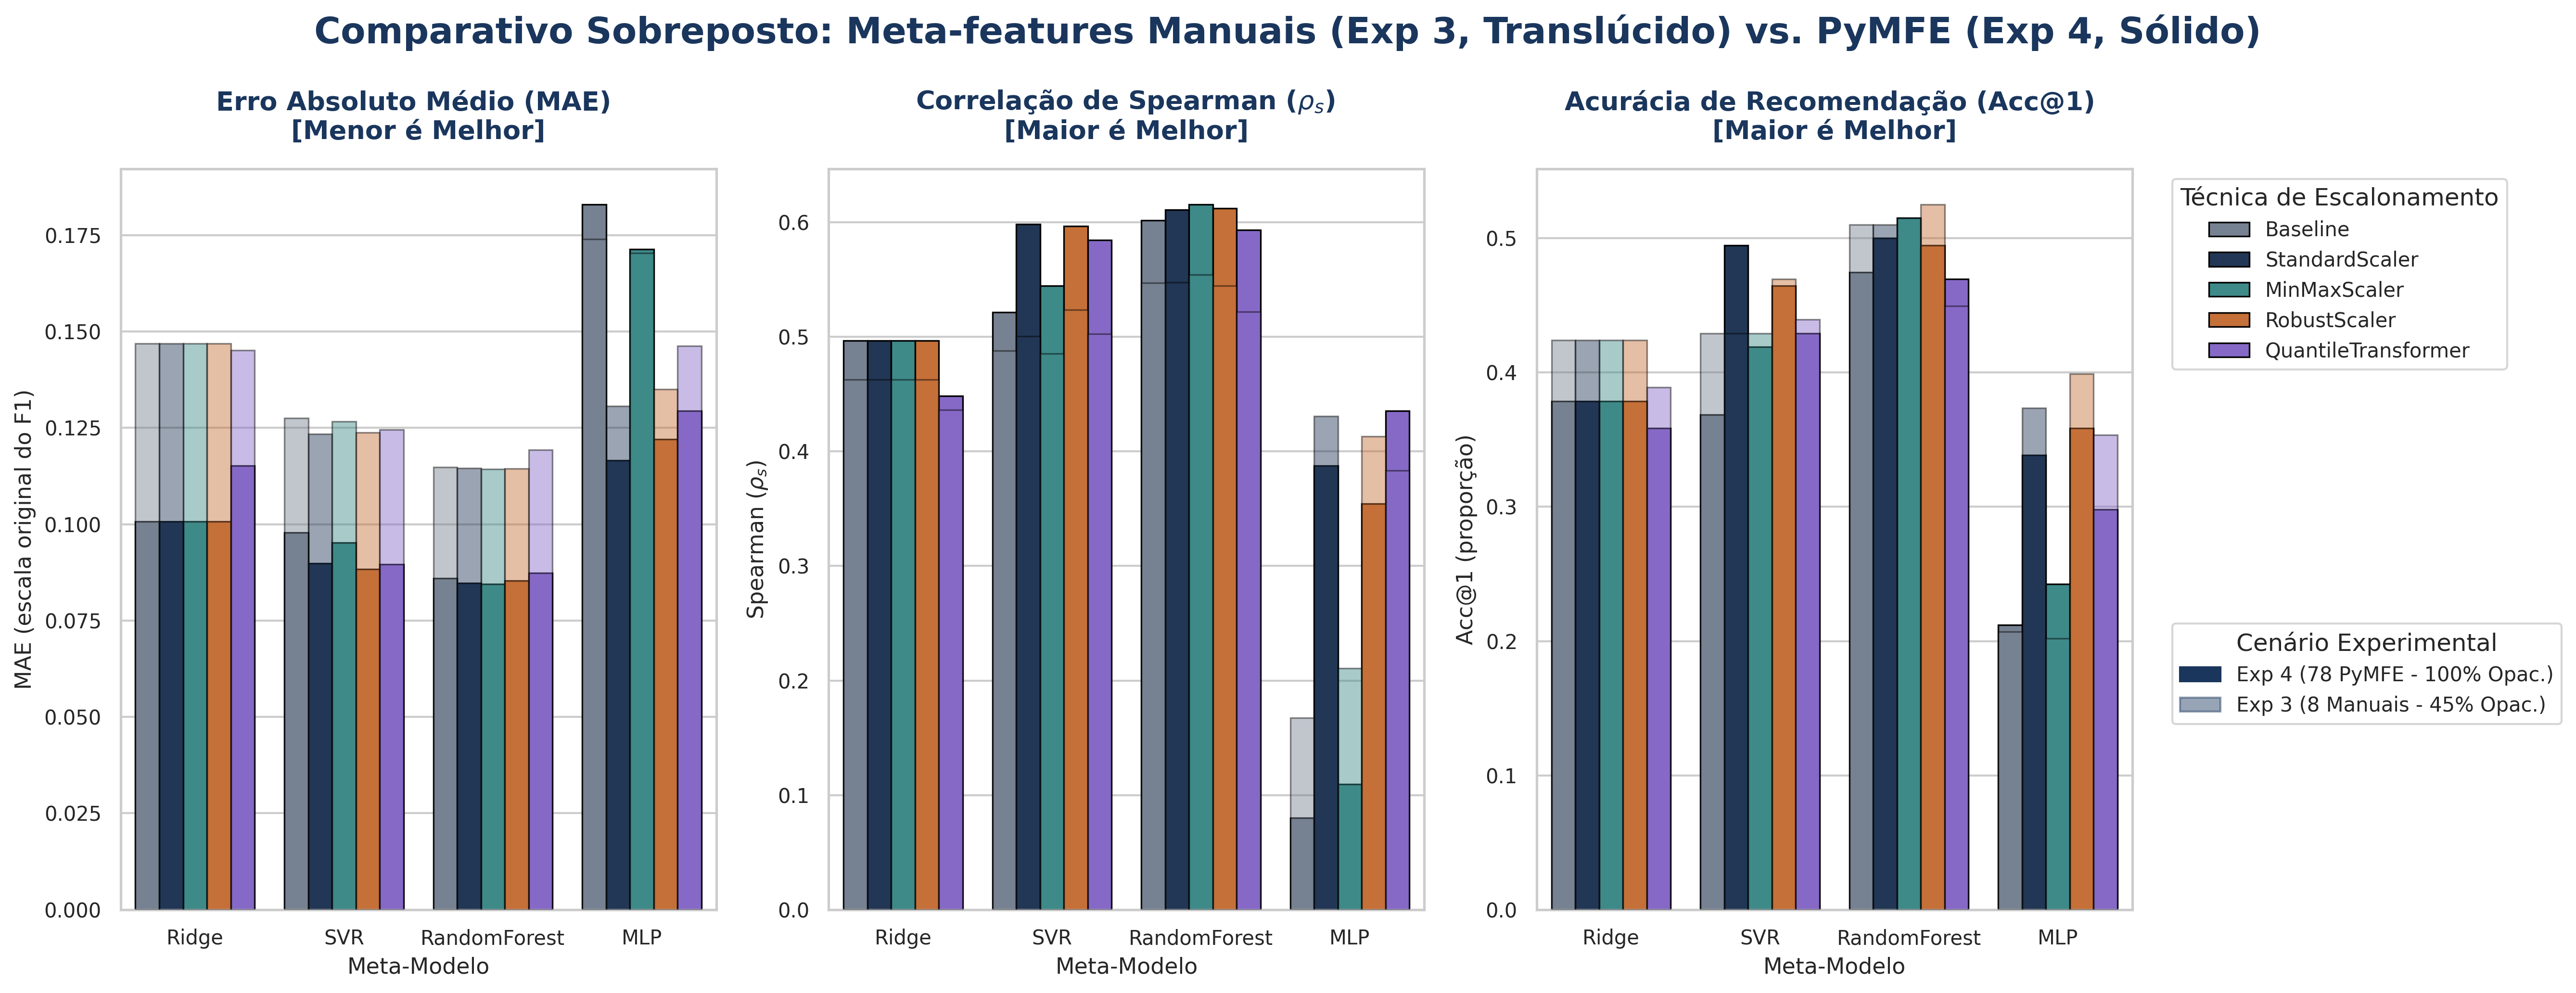
\includegraphics[width=0.82\textwidth]{figures/comparativo_sobreposto.png}
  \vspace{-0.1cm}
  \begin{exampleblock}{O Impacto da Riqueza de Meta-features}
    A transição das 8 features manuais (translúcido) para as 78 features do PyMFE (sólido) reduziu o MAE e aumentou a Spearman em todos os meta-modelos.
  \end{exampleblock}
\end{frame}

% Slide 10: Resultados - O Colapso do MLP
\begin{frame}{Resultados: O Colapso e Recuperação do MLP}
  \begin{columns}[T]
    \begin{column}{0.45\textwidth}
      \begin{block}{Colapso no Baseline}
        \small
        \begin{itemize}
          \item Sem centralização de escala, o MLP \textbf{colapsa} em dados reais.
          \item A Spearman cai a \textbf{0.080} e Acc@1 fica em \textbf{21.2\%} (pior que o acaso).
          \item Causa: Gradientes instáveis e saturação das ativações devido à alta dispersão.
        \end{itemize}
      \end{block}
      \begin{block}{Recuperação pelos Scalers}
        \small
        \begin{itemize}
          \item \textbf{Standard/RobustScaler} evitam o colapso: MAE reduz em \textbf{36.3\%} e Spearman sobe para \textbf{0.38 - 0.43}.
        \end{itemize}
      \end{block}
    \end{column}
    
    \begin{column}{0.52\textwidth}
      \footnotesize
      \begin{table}
        \centering
        \caption{Desempenho do MLP nos Experimentos}
        \begin{tabular}{llccc}
          \toprule
          \textbf{Cenário} & \textbf{Scaler} & \textbf{MAE} & \textbf{Spearman} & \textbf{Acc@1} \\
          \midrule
          \multirow{2}{*}{Exp. 1} & Baseline & 0,147 & 0,274 & 0,320 \\
                                  & Robust   & \textbf{0,071} & \textbf{0,588} & \textbf{0,440} \\
          \midrule
          \multirow{2}{*}{Exp. 2} & Baseline & 0,179 & 0,034 & 0,125 \\
                                  & Robust   & \textbf{0,118} & \textbf{0,453} & \textbf{0,438} \\
          \midrule
          \multirow{2}{*}{Exp. 3} & Baseline & 0,174 & 0,167 & 0,207 \\
                                  & Standard & \textbf{0,131} & \textbf{0,431} & \textbf{0,374} \\
          \midrule
          \multirow{2}{*}{Exp. 4} & Baseline & 0,183 & 0,080 & 0,212 \\
                                  & Robust   & \textbf{0,122} & 0,354 & \textbf{0,359} \\
          \bottomrule
        \end{tabular}
      \end{table}
    \end{column}
  \end{columns}
\end{frame}

% Slide 11: Resultados - Ridge, SVR e Random Forest
\begin{frame}{Resultados: Ridge, SVR e Random Forest}
  \begin{columns}[T]
    \begin{column}{0.32\textwidth}
      \begin{block}{Ridge (Linear)}
        \footnotesize
        \begin{itemize}
          \item \textbf{Matematicamente invariante} às transformações lineares no alvo.
          \item Resultados idênticos para Standard, Min-Max e Robust.
          \item O erro absoluto piora com o QuantileTransformer ($\Delta = +0,0145$).
        \end{itemize}
      \end{block}
    \end{column}
    
    \begin{column}{0.32\textwidth}
      \begin{block}{SVR (Kernel RBF)}
        \footnotesize
        \begin{itemize}
          \item Apresenta \textbf{melhora altamente significativa} ($p < 10^{-10}$) com escalonamento.
          \item O RobustScaler minimizou o MAE para \textbf{0.0884}.
          \item O StandardScaler maximizou a Spearman (\textbf{0.5982}) e o Acc@1 (\textbf{49.5\%}).
        \end{itemize}
      \end{block}
    \end{column}
    
    \begin{column}{0.32\textwidth}
      \begin{block}{Random Forest}
        \footnotesize
        \begin{itemize}
          \item \textbf{Invariante a escalas lineares:} MAE variou residualmente ($\approx 0.0015$) sem diferença estatística ($p = 0.333$).
          \item O MinMaxScaler apresentou o melhor resultado global ($\rho_s = \mathbf{0.6157}$, Acc@1 = $\mathbf{51.5\%}$).
        \end{itemize}
      \end{block}
    \end{column}
  \end{columns}
\end{frame}

% Slide 12: Validação Estatística - Teste de Friedman
\begin{frame}{Validação Estatística: Teste de Friedman}
  \begin{columns}[T]
    \begin{column}{0.58\textwidth}
      \small
      O teste de Friedman avalia se há diferença estatisticamente significativa no MAE ao variarmos as técnicas de escalonamento ($\alpha = 0,05$).
      \vspace{0.1cm}
      \begin{table}
        \centering
        \caption{Resultados do Teste de Friedman (Exp. 2, 3 e 4)}
        \tiny
        \begin{tabular}{llccl}
          \toprule
          \textbf{Experimento} & \textbf{Meta-Modelo} & \textbf{$\chi^2$} & \textbf{$p$-value} & \textbf{Decisão} \\
          \midrule
          \multirow{4}{*}{Exp. 2 (144 ds)}
           & Ridge        & 3,04            & 0,551            & Não significativo \\
           & SVR          & 8,37            & 0,079            & Não significativo \\
           & Random Forest & 5,41           & 0,248            & Não significativo \\
           & MLP          & \textbf{148,72} & $\mathbf{3{,}8 \times 10^{-31}}$ & \textbf{Significativo} \\
          \midrule
          \multirow{4}{*}{Exp. 3 (200 ds)}
           & Ridge        & 1,61            & 0,807            & Não significativo \\
           & SVR          & 3,41            & 0,491            & Não significativo \\
           & Random Forest & 0,34           & 0,987            & Não significativo \\
           & MLP          & \textbf{110,71} & $\mathbf{5{,}1 \times 10^{-23}}$ & \textbf{Significativo} \\
          \midrule
          \multirow{4}{*}{Exp. 4 (PyMFE)}
           & Ridge        & \textbf{22,38}  & $\mathbf{1{,}7 \times 10^{-4}}$  & \textbf{Significativo} \\
           & SVR          & \textbf{53,92}  & $\mathbf{5{,}5 \times 10^{-11}}$ & \textbf{Significativo} \\
           & Random Forest & 4,58           & 0,333            & Não significativo \\
           & MLP          & \textbf{278,02} & $\mathbf{5{,}9 \times 10^{-59}}$ & \textbf{Significativo} \\
          \bottomrule
        \end{tabular}
      \end{table}
    \end{column}
    
    \begin{column}{0.38\textwidth}
      \begin{block}{Evolução da Significância}
        \footnotesize
        \begin{itemize}
          \item \textbf{MLP}: Único modelo com sensibilidade estatística em todos os cenários reais (Exp. 2, 3 e 4).
          \item \textbf{Exp. 2 e 3}: Baixo volume de features manuais impediu a detecção de significância no SVR e Ridge.
          \item \textbf{Exp. 4 (PyMFE)}: O enriquecimento de entrada deu maior poder estatístico, revelando a sensibilidade do \textbf{SVR} e \textbf{Ridge}.
          \item \textbf{Random Forest}: Consistente e insensível em todos os cenários.
        \end{itemize}
      \end{block}
    \end{column}
  \end{columns}
\end{frame}

% Slide 13: Discussão: Paradoxo do QuantileTransformer
\begin{frame}{Discussão: O Paradoxo do QuantileTransformer}
  \begin{columns}[T]
    \begin{column}{0.5\textwidth}
      \begin{block}{Efeito de Distorção de Rank}
        \small
        \begin{itemize}
          \item O QT mapeia dados de forma não-linear para forçar normalidade.
          \item Embora minimize o MAE em alguns casos, ele \textbf{distorce a ordem relativa} dos algoritmos base.
          \item \textbf{Impacto:} Queda generalizada na acurácia Acc@1 para Ridge, SVR e RF.
        \end{itemize}
      \end{block}
    \end{column}
    
    \begin{column}{0.45\textwidth}
      \begin{alertblock}{O Caso Particular do MLP}
        \small
        \begin{itemize}
          \item No Experimento 4 (PyMFE), o QT foi o escalonador que obteve a \textbf{maior Spearman} para o MLP ($\rho_s = \mathbf{0,4355}$).
          \item \textbf{Explicação:} Em espaços densos de features, a normalização de alvo por quantis pode favorecer a correlação de rank do MLP.
        \end{itemize}
      \end{alertblock}
    \end{column}
  \end{columns}
  \vspace{0.2cm}
  \begin{exampleblock}{Recomendação Prática}
    Evitar o uso do QuantileTransformer se o objetivo do sistema for recomendar o melhor algoritmo (Acc@1).
  \end{exampleblock}
\end{frame}

% Slide 14: Conclusões e Recomendações
\begin{frame}{Conclusões e Recomendações}
  \begin{itemize}
    \item \textbf{Hipóteses Validadas:} A sensibilidade depende fortemente da arquitetura. Árvores são robustas; gradientes/kernel são sensíveis.
    \item \textbf{Riqueza de Features:} O uso do PyMFE foi crucial para reduzir erros absolutos.
    \item \textbf{Recomendação Prática:} Usar \textbf{RobustScaler} como padrão seguro para modelos sensíveis.
  \end{itemize}
  
  \vspace{0.1cm}
  
  \begin{table}
    \centering
    \caption{Guia de Recomendação de Escalonamento do Meta-Alvo}
    \footnotesize
    \begin{tabular}{lll}
      \toprule
      \textbf{Meta-Modelo} & \textbf{Objetivo do Sistema} & \textbf{Escalonador Recomendado} \\
      \midrule
      \textbf{Random Forest} & Qualquer Objetivo & \textbf{Baseline (Sem)} ou \textbf{MinMaxScaler} \\
      \multirow{2}{*}{\textbf{SVR}} & Maximizar Recomendação (Acc@1) & \textbf{StandardScaler} \\
                            & Minimizar Erro Absoluto (MAE) & \textbf{RobustScaler} \\
      \multirow{2}{*}{\textbf{MLP}} & Maximizar Recomendação (Acc@1) & \textbf{RobustScaler} \\
                            & Minimizar Erro Absoluto (MAE) & \textbf{StandardScaler} \\
      \midrule
      \textbf{Todos} & Evitar Deformar Rankings & \textcolor{red}{\textbf{X}} \textbf{Evitar QuantileTransformer para Acc@1} \\
      \textbf{MLP} & Evitar Erros Numéricos & \textcolor{red}{\textbf{X}} \textbf{Evitar MinMaxScaler e Baseline} \\
      \bottomrule
    \end{tabular}
  \end{table}
\end{frame}

\end{document}
